\chapter{Project Information}
Safe and secure home entry without the hassle of keys requires the development of a deadbolt whose locking and unlocking is controlled via PIN entry. The convenience of personalized PIN numbers for all users and the possibility of control through a mobile app would make home security easy.

The objective of the product is to provide convenience without sacrificing security. The scope of the proposed solution includes a deadbolt control mechanism, a method of confirming user identity via personal identification number, and possible development of wireless connectivity to provide remote access to the lock.


\section{Features}
This project is an Internet of Things (IoT) deadbolt. Containing an LCD display, keypad, and mobile application for additional features. This will allow the user to enter the pin through the onboard keyboard or send the pin through WiFi using Message Queuing Telemetry Transport (MQTT). Allowing the user to unlock the deadbolt from anywhere in the world along with entering the pin on the device.
Since this is still in development and this is the first release the lock currently only has a standard home screen, servo control, and a mobile application to control the locking/unlocking by sending a default pin.

\section{Screenshots}
The following two images are screenshots of the system in an unlocked state and a locked state. The first image is of the system locked. The second is an image of the system unlocked. 
\begin{figure}[htb]
    \begin{center}
        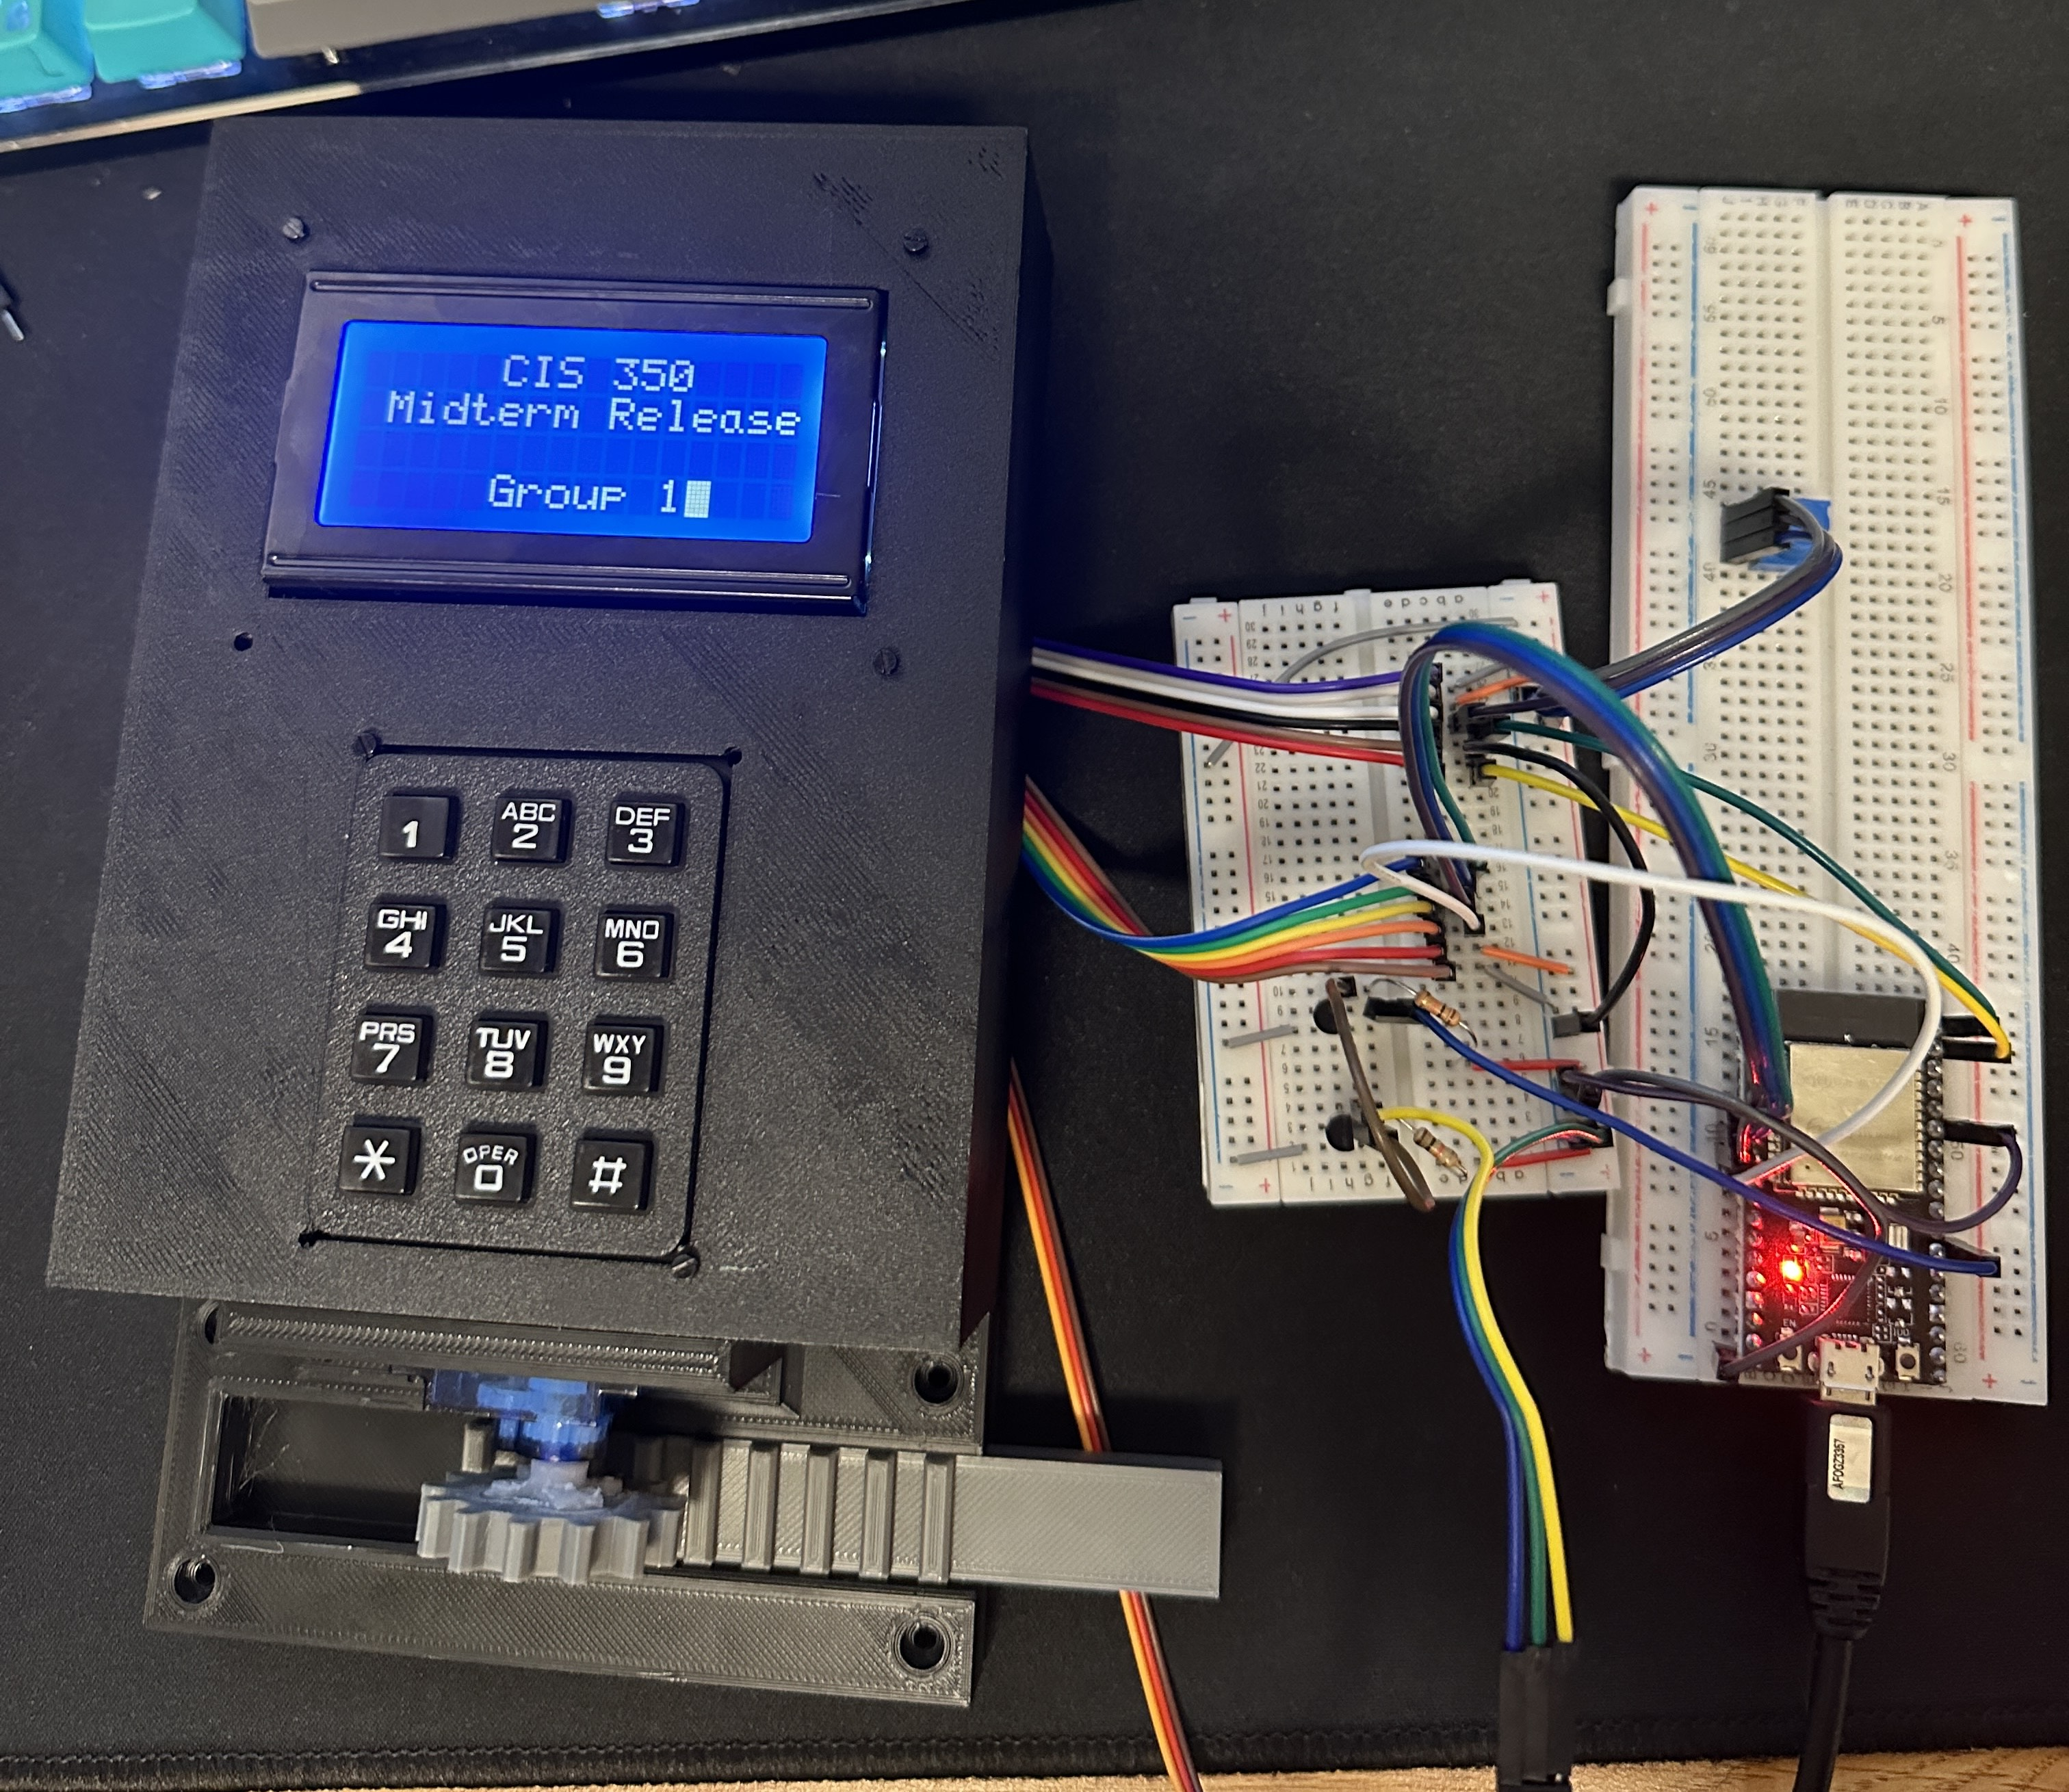
\includegraphics[width = \textwidth]{Images/Screenshot_of_system_locked.jpg}
        \caption{Image of system locked}
        \label{fig: Locked System}
    \end{center}
\end{figure}

\begin{figure}[htb]
    \begin{center}
        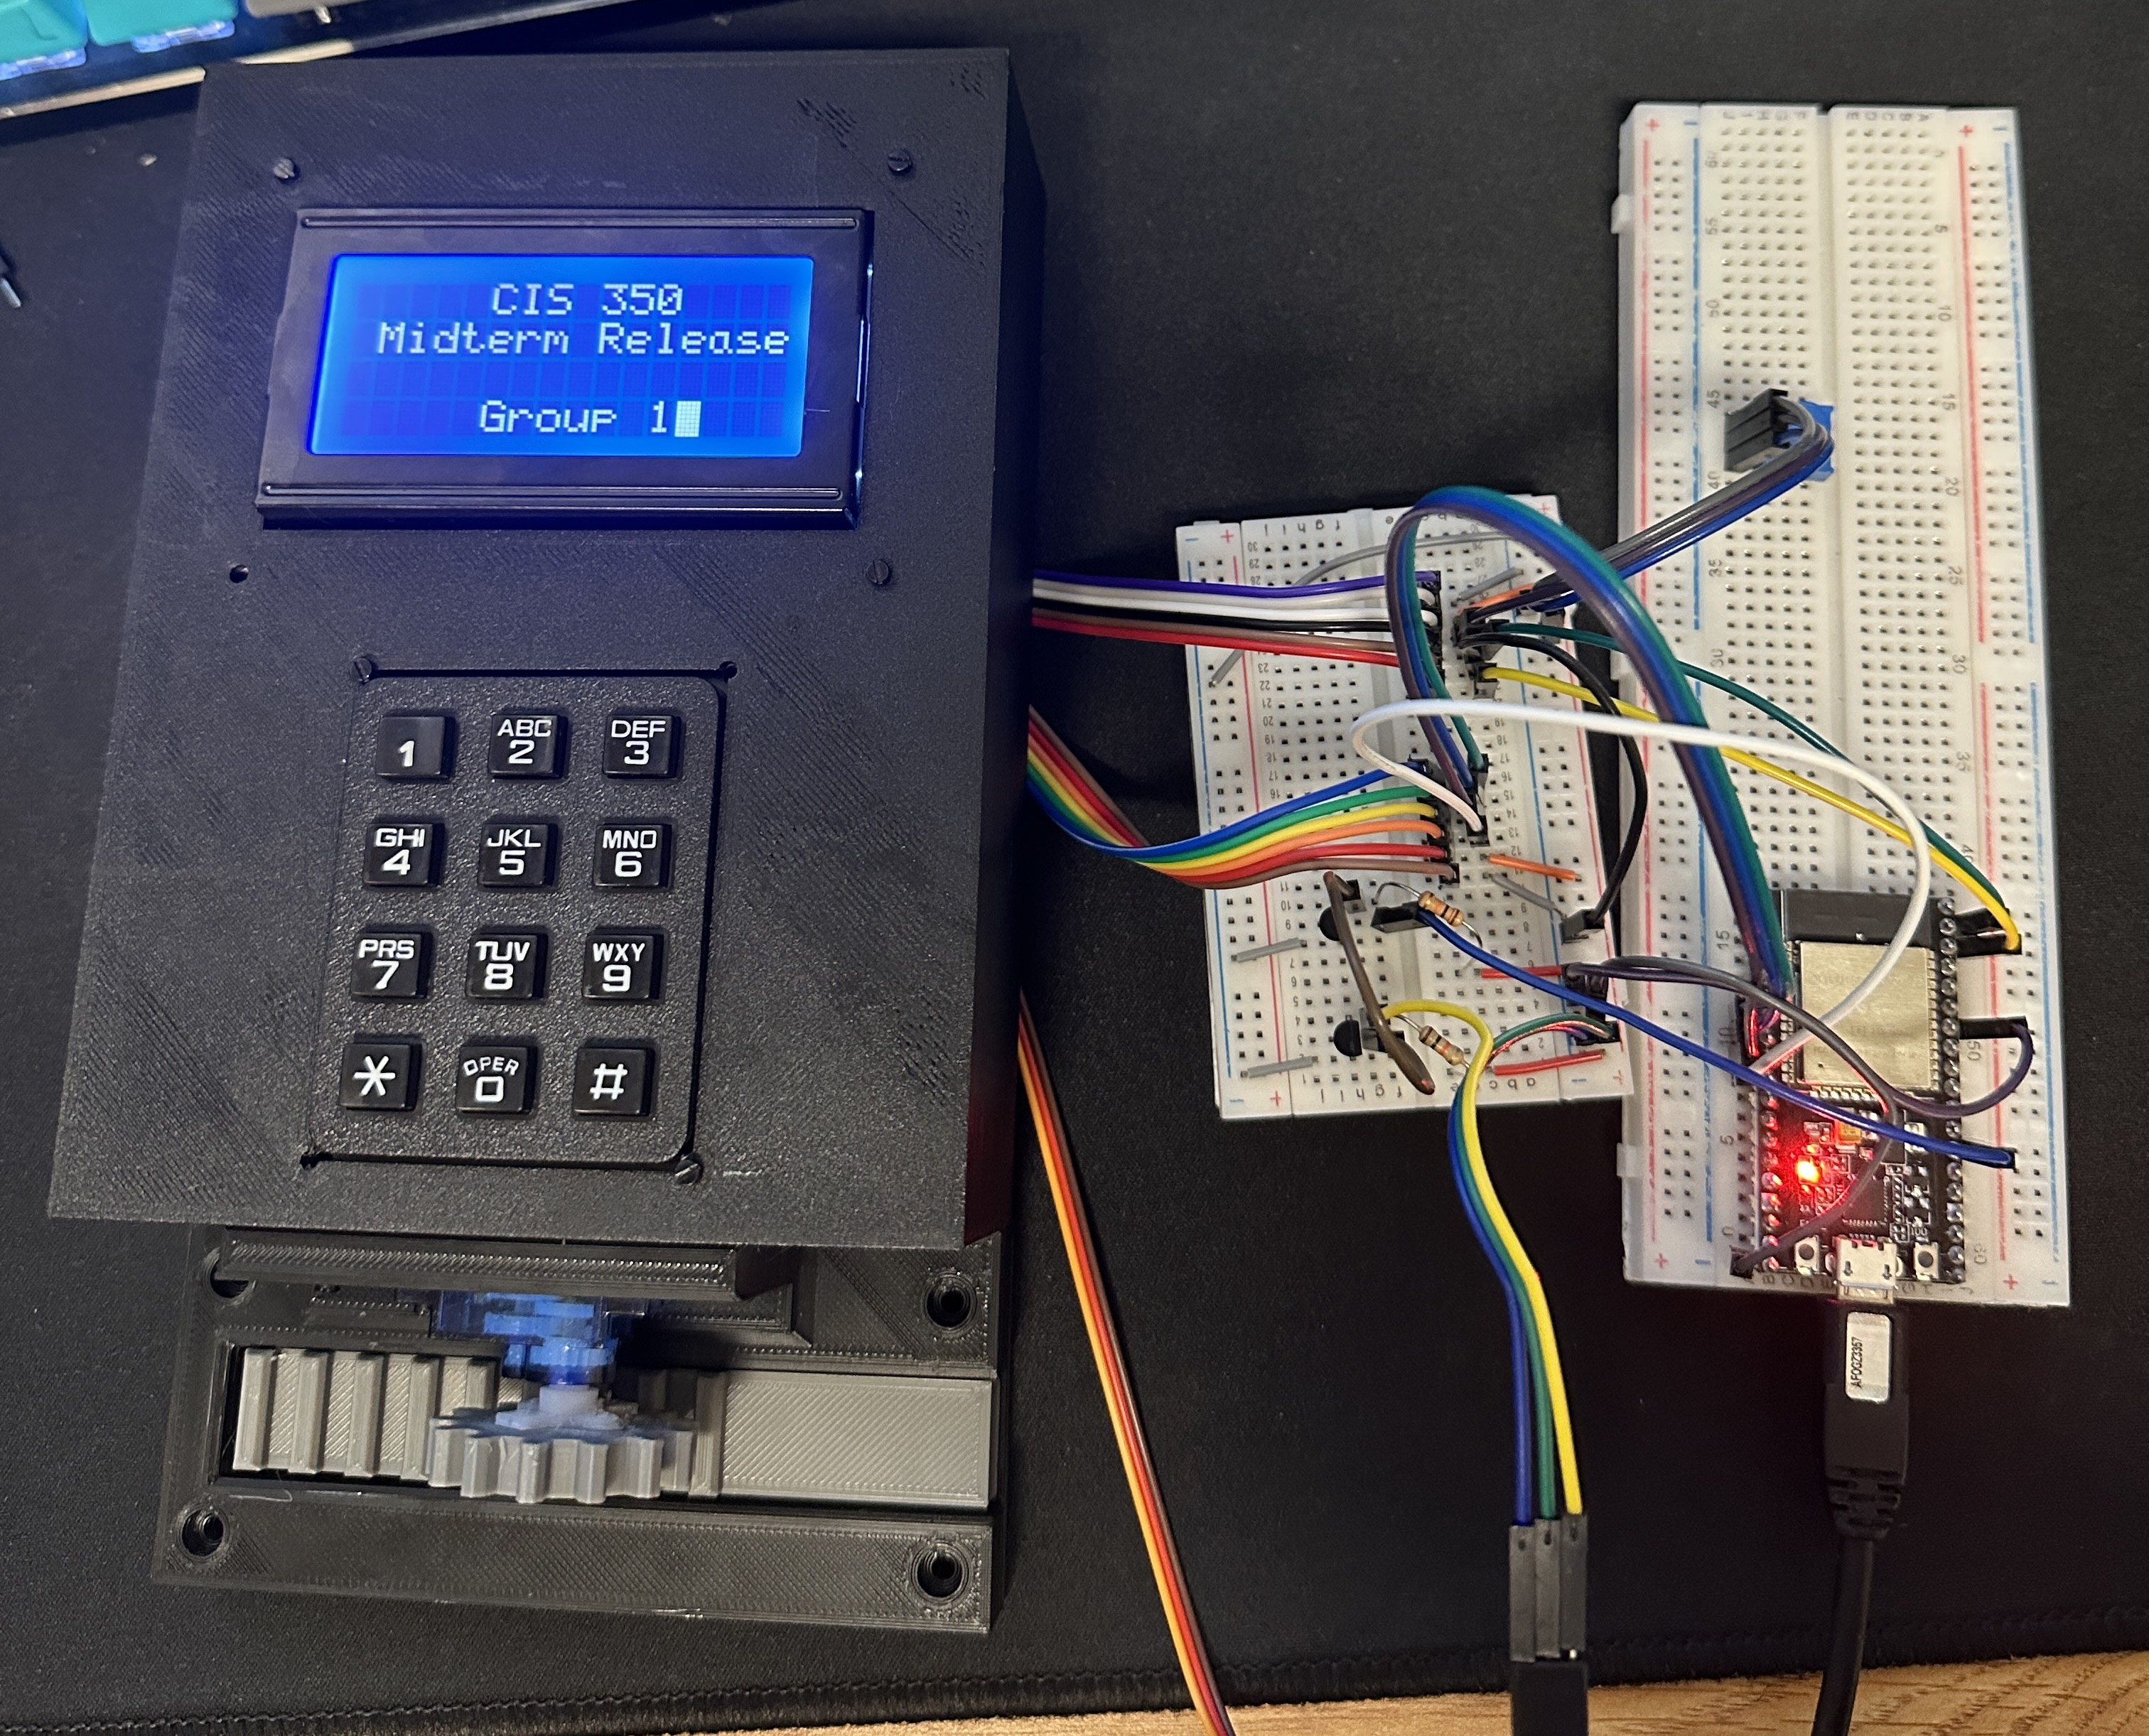
\includegraphics[width = \textwidth]{Images/Screenshot_of_system_unlocked.jpg}
        \caption{Image of system unlocked}
        \label{fig: Unlocked system}
    \end{center}
\end{figure}